\section{Measuring Third-Party Data Dependence}
\label{sec:measurement}

\subsection{Text Corpus}

The text corpus consists of the 2019 annual reports of the sample firms. We use annual reports rather than earnings-call transcripts for three reasons. First, annual reports follow a standardized disclosure format and cover the full sample; earnings-call transcripts for Chinese digital firms are incomplete in 2019. Second, the ``Business Overview'' and ``Management Discussion and Analysis'' sections describe business models, customer structure, traffic sources, advertising, data partnerships, and platform dependence, which map directly to the four dimensions of third-party data dependence. Third, the 2019 reports were published in early 2020, before ATT and PIPL, and are therefore predetermined with respect to the shock.

For each PDF, we locate the main body of the business overview or management discussion section and retain a 60,000-character window. We remove page headers, footers, and page numbers. If a firm uses a different heading, we use the main-text start as the anchor. The final corpus contains 298 parseable reports with an average length of about 55,500 characters.

\subsection{Lexicon and Index Construction}

The lexicon has six categories. Category A covers third-party data acquisition, including ``third-party data'', ``purchased data'', ``data procurement'', ``data supplier'', ``data transaction'', ``data sharing'', and ``data interface''. Category B covers third-party traffic and advertising, including ``traffic purchase'', ``customer acquisition cost'', ``ad buying'', ``advertising placement'', ``precision marketing'', ``programmatic advertising'', ``information-flow advertising'', ``ad network'', and ``app distribution''. Category C covers user profiling and tracking, including ``user profile'', ``tag system'', ``cross-app'', ``cross-device'', ``device identifier'', ``IDFA'', ``OAID'', ``targeted placement'', and ``personalized recommendation''. Category D covers platform dependence, including ``third-party platform'', ``open platform'', ``app store'', ``iOS'', ``WeChat mini-program'', ``Douyin'', ``Kuaishou'', ``Xiaohongshu'', ``Ocean Engine'', and ``Alimama''. Category E covers first-party data capability, including ``owned data'', ``first-party data'', ``private-domain traffic'', ``membership system'', ``user community'', ``WeCom'', ``CRM'', ``data middle platform'', and ``CDP''. Category F covers generic digitalization, including ``digital transformation'', ``cloud computing'', ``big data'', ``artificial intelligence'', ``Internet of Things'', ``blockchain'', ``5G'', ``industrial internet'', and ``large language model''.

Term counts use a longest-match rule: within a character span, the longest term is matched first, so nested terms such as ``data service'' and ``data service provider'' are not double counted. Let $N_{ic}$ be the count of category $c$ for firm $i$ and $L_i$ the text length. The category intensity is $10{,}000\times N_{ic}/L_i$. The TDDI is the equal-weighted average of the four treatment categories, log-transformed and standardized:
\begin{equation}
\text{TDDI}_i=\text{Std}\left[\ln\left(1+\frac{1}{4}\sum_{c=A}^{D}\frac{10{,}000N_{ic}}{L_i}\right)\right].
\label{eq:tddi}
\end{equation}
Equal weighting prevents categories with more terms from dominating the index. The log transformation limits the influence of a small number of firms with very high disclosure frequency. FPDCI and the generic digitalization index are constructed in the same way from categories E and F. Appendix Table 
ef{tab:lexicon} lists the six constructs and representative terms.

\subsection{Reliability and Construct Validity}

Table \ref{tab:validity} reports the reliability and construct validity of the TDDI. We split the A--D terms into two random halves, compute the two half-indices, and correlate them across firms. Repeating the split 200 times yields a mean correlation of 0.677; the Spearman--Brown correction is 0.807. The index therefore captures a stable firm characteristic rather than idiosyncratic wording.

Figure \ref{fig:tddi} reports the industry distribution. Advertising and marketing has the highest mean TDDI (1.31), followed by internet e-commerce (0.52) and gaming (0.20); education has the lowest mean ($-0.68$). The ordering matches the intuition about who relies on third-party data: advertising firms buy traffic and audiences, e-commerce firms depend on platform referral and cross-site tracking, and education firms rely more on offline and brand-based acquisition.

The TDDI correlates 0.323 with the generic digitalization index. Generic digitalization captures whether a firm is digital; the TDDI captures whether a firm depends on external data. The two constructs are related but not equivalent, so the TDDI is not absorbed by a generic digitalization narrative. Correlations with the selling-expense ratio, gross margin, and ROA are close to zero (Panel A of Table \ref{tab:validity}). This pattern is informative: the TDDI measures data dependence, not advertising intensity. A firm can depend on third-party data through procurement, interfaces, or platform fees without reporting high advertising expenses. The economic validity of the TDDI therefore rests on its split-half reliability, its industry pattern, and its ability to predict the valuation response to the privacy shock in Section 8.

\begin{figure}[htbp]
\centering
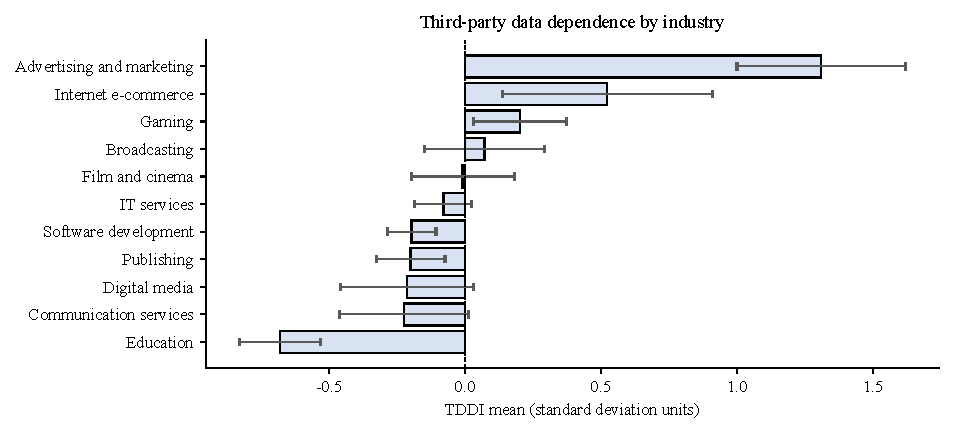
\includegraphics[width=0.95\textwidth]{fig2_tddi_industry.pdf}
\caption{Average TDDI by industry. Bars report the mean TDDI; error bars are standard errors of the mean. The index is standardized to mean zero and unit standard deviation. The sample contains 298 Chinese A-share digital firms; the index is constructed from 2019 annual-report texts.}
\label{fig:tddi}
\end{figure}

\begin{table}[htbp]
\centering
\small
\caption{Construct validity and reliability of the TDDI.}
\label{tab:validity}
\begin{threeparttable}
\begin{tabular}{lccc}
\toprule
 & Pearson correlation & Spearman correlation & Observations \\
\midrule
\multicolumn{4}{l}{Panel A: Correlations with external proxies and a placebo} \\
Selling-expense ratio & -0.005 & 0.119 & 288 \\
Gross margin & 0.031 & 0.120 & 288 \\
ROA & 0.035 & 0.007 & 289 \\
Firm size & 0.116 & 0.188 & 289 \\
Leverage & -0.001 & -0.067 & 289 \\
Generic digitalization & 0.323 & 0.370 & 298 \\
\midrule
\multicolumn{4}{l}{Panel B: Reliability} \\
Split-half correlation (mean of 200 random splits) & 0.677 & & 298 \\
Spearman--Brown corrected correlation & 0.807 & & 298 \\
\bottomrule
\end{tabular}
\begin{tablenotes}[flushleft]
\footnotesize
\item Notes: External proxies are 2019 firm-level averages. The TDDI is constructed from 2019 annual-report texts. The generic digitalization index is the standardized frequency of category F terms and serves as a placebo. The split-half correlation randomly divides the A--D terms into two halves and correlates the resulting indices across firms.
\end{tablenotes}
\end{threeparttable}
\end{table}

